\chapter{Aufbau}
Die Benutzeroberfläche wird durch Screens, Components und StyleSheets zusammengesetzt. Screens sind
komplette Ansichten, sie belegen den ganzen Bildschirm des Geräts. Alle Elemente in einem Screen
werden durch Components aufgebaut. Den Feinschliff erledigen die StyleSheets, in ihnen werden alle
Informationen gespeichert, welche für die Positionierung, Größe, Farbe, usw. von Komponenten wichtig
sind.

\section{Screens}
In unserer App wollen wir Informationen für den Benutzer verständlich darstellen. Es würde keinen
Sinn machen alle Informationen auf die gleiche Seite zu schreiben, eine logische Gliederung der App
ist daher sehr wichtig. Screens sind im Grunde nur React-Komponenten; sie werden aus mehreren
kleineren Komponenten zusammengebaut.

\section{Arten von Screens}
In Apps gibt es eigentlich nicht so viele Arten von Screens, hier die häufigsten Anwendungsfälle im
Überblick:

\subsection{Listen}
Listen-Screens sind dafür da, um mehrere Datensätze untereinander oder nebeneinander darzustellen.
Dafür wird über jedes Element in einer Liste iteriert und an eine Komponente weitergegeben, welche
anschließend die Daten aufbereitet und darstellt.

\subsection{Details}
Nachdem man jedes Element aufgelistet hat, sollte es noch möglich sein ein Element genauer zu
betrachten bzw. alle Informationen anzuzeigen, welche nicht im Überblick der Liste Platz haben.

\subsection{Formulare}
In Formularen kann der Benutzer Informationen in die App eintragen, welche dann per \textbf{HTTP} an
das Backend geschickt werden.
\section{Komponenten}
Komponenten, die in vielen anderen Komponenten gebraucht werden, werden bei uns im Ordner
root/components/common gespeichert. Andere Komponenten werden im components-Ordner nach ihrem
zugehörigen Screen getrennt.

\subsection{Snippets}
Um Komponenten schneller erzeugen zu können gibt es in Visual Studio Code Snippets, welche immer den
selben Code generieren.

\begin{figure}[H]
  \begin{center}
    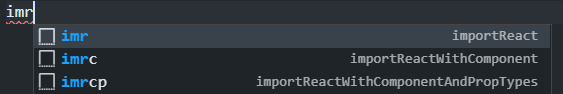
\includegraphics[width=0.5\textwidth]{Mobile/VSSnippets.png}
    \caption{Beispiel für ein Snippet}
  \end{center}
\end{figure}

\begin{figure}[H]
  \begin{center}
    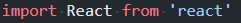
\includegraphics[width=0.5\textwidth]{Mobile/VSSnippetsIMR.png}
    \caption{Vom Snippet erzeugter Code}
  \end{center}
\end{figure}

Da jede Komponente in unserer App ähnlich aufgebaut ist und damit wir nicht jedes mal den gleichen
Code schreiben müssen, habe ich ein eigenes Snippet erstellt. Die Abkürzung rnfec steht hierbei für
React Native Functional Component Export Custom und erzeugt folgenden Code:

\begin{lstlisting}
import React from 'react'
import { View } from 'react-native'
import Text from '@components/common/Text';

const Test = () => {
  return (
    <View>
      <Text></Text>
    </View>
  )
}

export default Test
\end{lstlisting}

Der Name der Komponente wird hierbei vom Dateinamen abgeleitet. Eine Besonderheit, die auffällt, ist
das Import-Statement von Text. Das Verwenden von Alias-Paths wird durch das Babel-Plugin
"module-resolver" möglich gemacht.

\newpage
\subsection{Text}
In React Native gibt es keinen sicheren Weg, um allen Text-Komponenten automatisch eine Font
zuzuweisen, deswegen wird in unserer App immer eine eigene Text-Komponente verwendet. Diese wird
auch beim Erzeugen von neuen Komponenten automatisch eingebunden, damit nicht versehentlich doch die
falsche Komponente verwendet wird.

\begin{lstlisting}
import React from 'react';
import { Text, StyleSheet } from 'react-native';
import colors from '../../styles/Colors';

const CustomText = ({ style, children }) => (
  <Text style={[styles.defaultStyle, style]}>{children}</Text>
);

const styles = StyleSheet.create({
  defaultStyle: {
    fontFamily: 'Poppins-Regular',
    color: colors.text,
  },
});

export default CustomText;
\end{lstlisting}

Alle Kinder dieser Komponente werden dann direkt in den Text eingebunden und, sollte man noch ein
style-Property an die Komponente übergeben wird der Standard-Style überschrieben.

\newpage
\subsection{Button}
Auch der Button-Component von React Native lässt sich leicht nachbauen.

\begin{lstlisting}
import React from 'react';
import { Pressable } from 'react-native';
import MaterialCommunityIcons from 'react-native-vector-icons/MaterialCommunityIcons';
import Ionicons from 'react-native-vector-icons/Ionicons';
import MaterialIcons from 'react-native-vector-icons/MaterialIcons';

import Text from './Text';
import styles from '@styles/GlobalStyles';

const Button = ({
  onPress,
  title,
  icon,
  iconType,
  style,
  iconSize = 24,
}) => (
  <Pressable
    onPress={onPress}
    style={[styles.buttonContainer, styles.shadow, style]}
  >
    <Text style={styles.buttonText}>{title}</Text>

    {icon && iconType === 'mci' && (
      <MaterialCommunityIcons
        name={icon}
        size={iconSize}
        color={styles.buttonText.color}
      />
    )}
    {icon && iconType === 'mi' && (
      <MaterialIcons
        name={icon}
        size={iconSize}
        color={styles.buttonText.color}
      />
    )}
    {icon && iconType === 'ii' && (
      <Ionicons name={icon} size={iconSize} color={styles.buttonText.color} />
    )}
  </Pressable>
);

export default Button;
\end{lstlisting}

Die Funktion, welche beim Drücken aufgerufen werden soll, wird der Komponente als onPress übergeben.
Sollte das Prop icon leer sein, wird kein Icon gerendert, andernfalls wird noch überprüft, welche
Art von Icon verwendet werden soll. Die Icons werden nämlich von mehreren Anbietern bereitgestellt.

\newpage
\subsection{TextInput}
Auch die Komponente TextInput wird von uns überschrieben. Sie besteht zusätzlich immer aus einem
Icon auf der linken Seite. Je nach dem, ob der Input gerade bearbeitet wird, wird die Farbe
verändert. Solle bei der Textüberprüfung ein Fehler auftreten, so wird die Komponente rot gefärbt.

\begin{figure}[H]
  \begin{center}
    
\includegraphics[width=0.5\textwidth]{Mobile/TextInput/unfocused.png}
    \caption{Der TextInput für die Email am Login-Screen}
  \end{center}
\end{figure}

\begin{figure}[H]
  \begin{center}
    
\includegraphics[width=0.5\textwidth]{Mobile/TextInput/focused.png}
    \caption{TextInput ausgewählt}
  \end{center}
\end{figure}

% \begin{figure}[H]
%   \begin{center}
%     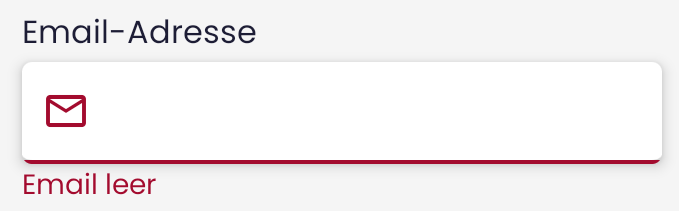
\includegraphics[width=0.5\textwidth]{Mobile/TextInput/error1.png}
%     \caption{Pflichtfeld leer}
%   \end{center}
% \end{figure}

\begin{figure}[H]
  \begin{center}
    
\includegraphics[width=0.5\textwidth]{Mobile/TextInput/error2.png}
    \caption{Fehlerhafte Eingabe}
  \end{center}
\end{figure}

\begin{figure}[H]
  \begin{center}
    
\includegraphics[width=0.5\textwidth]{Mobile/TextInput/valid.png}
    \caption{Korrekte Eingabe}
  \end{center}
\end{figure}
\newpage
\section{Styles}
\subsection{Schriftart}
Durch den Common-Component \textbf{Text} können wir jedem Textfeld in der App eine einheitliche Schriftart
geben. Ich entschied mich für die Font Poppins \cite{poppins}.

\subsection{Farbwerte}
Alle Farben, die man in der App sehen kann, wurden in der Datei \textbf{Colors.js} in
\textbf{root/styles} festgelegt. So muss nicht, sollte sich das Design ändern müssen, in jedem
StyleSheet jede Farbe einzeln getauscht werden.

Die Hauptfarbe der App ist der wunderschöne Grünton Jade (\#00A86B), welchen ich durch die Webseite
color-name.com \cite{colorName} fand. Die Webseite MyColor.Space \cite{myColorSpace} erzeugt anhand
einer Farbe mehrere andere Farben, die gut dazu passen.

\subsection{Icons}
Die Bibliothek \textbf{react-native-vector-icons} \cite{reactNativeVectorIcons} war eine große Hilfe
bei der Erstellung des Designs, Icons sind nämlich der perfekte Weg, um Informationen auf wenig Platz
darzustellen, z.B. welche Funktion ein Knopf hat. Ich habe stets darauf geachtet diverse Icons von
verschiedenen Anbietern in die App einzubauen. Hauptsächlich verwende ich die
\textbf{MaterialCommunityIcons}, eine große Sammlung von Icons orientiert am Material Design, einer
Designsprache entwickelt von Google.

\newpage
\subsection{FlashMessage}
\begin{code}[htp]
\begin{lstlisting}[firstnumber=1,language=JavaScript, style=JSX]
const App = () => (
  ...
  <FlashMessage position="top" />
  ...
);

export default App;
\end{lstlisting}
\caption{React Component - FlashMessage-Komponente in root/App.js}
\end{code}

Die Komponente FlashMessage ist für Mitteilungen über Geschehnisse in der App zuständig, z.B.
Login fehlgeschlagen oder Login erfolgreich.

\begin{figure}[H]
  \begin{center}
    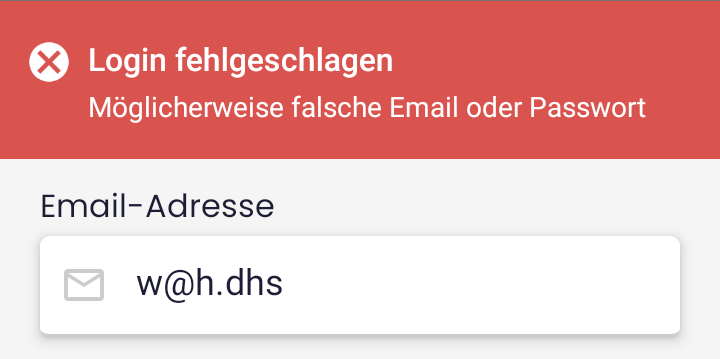
\includegraphics[width=0.5\textwidth]{Mobile/Auth/failed.png}
    \caption{Login-Informationen falsch}
  \end{center}
\end{figure}

\begin{figure}[H]
  \begin{center}
    
\includegraphics[width=0.5\textwidth]{Mobile/Auth/granted.png}
    \caption{Login-Informationen richtig}
  \end{center}
\end{figure}
